%%%%%%%%%%%%%%%%%%%% author.tex %%%%%%%%%%%%%%%%%%%%%%%%%%%%%%%%%%%
%
% sample root file for your "contribution" to a proceedings volume
%
% Use this file as a template for your own input.
%
%%%%%%%%%%%%%%%% Springer %%%%%%%%%%%%%%%%%%%%%%%%%%%%%%%%%%


\documentclass{svproc}
%
% RECOMMENDED %%%%%%%%%%%%%%%%%%%%%%%%%%%%%%%%%%%%%%%%%%%%%%%%%%%
%

% to typeset URLs, URIs, and DOIs
\usepackage{url}
\usepackage[utf8]{inputenc}
\usepackage{graphicx}
\def\UrlFont{\rmfamily}

\begin{document}
\mainmatter              % start of a contribution
%
\title{Person Following Robot Behavior Using Deep Learning}
%
%
\author{No author is given}
% \author{Ignacio Condés\inst{1} \and José María Cañas\inst{2}}
% %
% %
\institute{No institute is given}
% \institute{Universidad Rey Juan Carlos,
% 	\email{ignacio.condes.m@gmail.com},
% 	\and
% Universidad Rey Juan Carlos, \email{jmplaza@gsyc.urjc.es}}

\maketitle              % typeset the title of the contribution

\begin{abstract}
Human-robot interaction (HRI) is a field with growing impact as robot applications are entering into homes, supermarkets and general human environments. Person following is an interesting capability in HRI. This paper presents a new system for a robust person following behavior inside a robot. Its perception module addresses the person detection on images using a pretrained TensorFlow SSD \emph{Convolutional Neural Network} which provides \emph{robustness} even on tough lighting conditions. It also includes a face detector and a \emph{FaceNet} CNN to reidentify the target person. Care has been put to allow real-time operation. 
%A \emph{person tracker filter} has been included to alleviate the effect of false positives/negatives. It also extracts faces, which are also analyzed by a \emph{FaceNet} CNN to reidentify the tracked individual. 
%This perception module tells which person in the image has to be followed, even on poorly lightened scenarios. 
%It is combined with depth readings to obtain the relative position of the person. 
The control module implements two \emph{PID} controllers for a reactive smooth response, moving the robot towards the target person without distracting with other people around. The entire system has been experimentally validated on a real TurtleBot2 robot, with an Asus Xtion RGBD camera.
% We would like to encourage you to list your keywords within
% the abstract section using the \keywords{...} command.
\keywords{Computer Vision, neural networks, deep learning, robotic behavior}
\end{abstract}
%

%  ---- Intro ----
\section{Introduction}
%
In this project, we aim to establish a scope which covers two fields: \emph{robotics} and \emph{deep learning}.\\

In the last decades, robots have become a powerful allied to humans, as they are leveraged to perform all kind of tasks (hazardous explorations, personal assistance, cleaning, driving, \dots). However, we aim to design them to perform these tasks on the most autonomous way possible, which means not requiring to be controlled on every action (with exceptions, such as surgeon robots). This requires to provide robots a certain intelligence and capabilities to correctly trigger the most suitable action for each possible input stimulus. For this purpose, we can find multiple approaches for different problems (navigation, conversation, \dots).\\

Concretely, this article is dovetailed with \emph{Computer Vision}, which involves connecting cameras to a robot, and taking advantage of this on an autonomous way. Concretely, we will tackle the \emph{person following} challenge, which is based on a behavior governed by a person \emph{detection} system. Many approaches are already existing, such as color filters \cite{rocapal}, or disparities filtering. However, promising \emph{Deep Learning} techniques excel on their image processing variant, as they offer high quality results, accompanied by \emph{robustness} facing lighting issues (Fig. \ref{fig:intro_harsh_light}). This is the set of techniques we have used on this project, so we will describe the basis firstly.\\

\begin{figure}[h]
	\centering
	\includegraphics[width=2in]{images/light_ko_2}
	\caption{Harsh lighting situation for \emph{Computer Vision} algorithms.}
	\label{fig:intro_harsh_light}
\end{figure}


In the image detection quandary, the main objective is to determine \emph{presence and position} of a certain object in a given image. For this, we make use on this article of \emph{deep learning} techniques, concretely \emph{Convolutional Neural Networks} (CNNs).\\


This investigation has focused on exploring the synergies existing the two explained fields, making use of \emph{deep learning} to automatically command a robot to follow a determined person. This is achieved making use of two different modules: a \emph{perception} one, focused on the computer vision/deep learning tasks, and an \emph{actuation} module, which implements a case-based behavior, depending on what the perceptive part senses and computes. The designed system has been experimentally validated, as it will be seen on section \ref{sec:experiments}

% ---- State of the art ----
\section{State of the Art}
There are not any other techniques for the moment, we have invented robotics and deep learning entirely.

% ---- Infrastructure ----
\chapter{Infrastructure}

	This chapter is destined to a brief description of all the available hardware/software resources on which we will rely along the project.\\
 
\section{Hardware}
	\subsection{Sony EVI D100P camera}
	\label{sec:3_ptz}
		\begin{figure}[h]
			\centering
			\begin{subfigure}[h]{0.4\linewidth}
				\centering
				\includegraphics[width=1.6in]{images/ptz_front}
				\caption{Front side.}
			\end{subfigure}
			\qquad
			\begin{subfigure}[h]{0.4\linewidth}
				\centering
				\includegraphics[width=1.6in]{images/ptz_back}
				\caption{Back side.}
			\end{subfigure}
			\caption{Sony EVI D100P.}
			\label{fig:3_evi}
		\end{figure} 
		
		The first used hardware element is the Sony EVI D100P\footnote{\url{https://pro.sony/en_IN/products/ptz-network-cameras/evi-d100-d100p-pal-}}. It is a \emph{PTZ} cam (which stands for \emph{Pan Tilt Zoom}) which, originally thought and designed for videoconferences, is equipped with a bunch of precision servo motors. This allows it to be teleoperated, performing a soft and steady two-dimensional movement on demand:
		\begin{itemize}
			\item \emph{Pan:} horizontal movement. It can take values from $-100$ to $100$ degrees from the centered position. This movement can be performed at a certain speed, which can be set between $1$ and $24$.

			\item \emph{Tilt:} vertical movement. Its range goes from $-30$ to $30$, and the movement speed can be also varied between $1$ and $20$.
		\end{itemize}
		
		Something remarkable about this device is that it is bidirectional: we \textit{receive} images from its camera, and, at the same time, we \textit{send} it commands to move the motors.\\
		
		\begin{description}
			\item[Motors] 
			The low-level implementation of the movement commands is the \emph{VISCA} protocol, a proprietary solution from the manufacturer (Sony). It is received by the cam through a RS-232C (the traditional low-rate serial interface before USB spread), so we can connect it to a modern computer with a RS232-USB interface.
			
			However, the driver that controls this camera (\autoref{sec:3_evicam_driver}) does not offer support for a \emph{zoom} movement, but it is not very relevant for this application.\\
			
			\item[Video] 		As the video sensor is an analogue device, we need to convert its information to a digital format. We achieve this with a video capture device (\autoref{fig:3_dazzle}), which outputs digital video. This image flow is processed by a ROS driver (\autoref{sec:3_usb_cam}), that will be later explained.
			
			\begin{figure}[h]
				\centering
				\includegraphics[width=3in]{images/pinnacle_dazzle}
				\caption{Analogue-digital video converter (Pinnacle Dazzle).}
				\label{fig:3_dazzle}
			\end{figure}
			
			
		\end{description}

	
		We have to be careful on the movement commands (as it will be seen on \autoref{sec:follow_ptz}).\\

		This is the device we use on our experimental approach to the \emph{detection + robotic behavioral} node (\autoref{sec:follow_ptz}), where the only response is moving the camera.\\

	\subsection{Asus Xtion Pro Live}
		\label{sec:3_xtion}
		It is a RGBD (RGB + Depth) sensor, designed by Asus for interactive PC applications development purposes.

		\begin{figure}[h]
			\centering
			\includegraphics[width=0.4\linewidth]{images/xtion}
			\caption{Asus Xtion Pro Live. IR emitter (left), and RGB and IR lenses (right).}
			\label{fig:3_xtion}
		\end{figure}

		It counts on its left side with an IR (\emph{infrared}) light emitter, which radiates beams like a conventional light bulb (that's its function). On the right side, we can find two sensors:
		\begin{itemize}
			\item \emph{RGB sensor:} a regular digital camera, with a resolution up to 1280x1024 px.
			
			\item \emph{Depth sensor:} measures distance to objects by receiving the reflections of the IR beams that we have mentioned above. It maps, for each pixel, the distance to that reflection (in mm), stored as a 16-bit long value. Thus, we can obtain a depth image, with a resolution of 640x480 px (@ 30 fps).
		\end{itemize}

	We have used it as the visual source in the developed \emph{detection + robotic behavioral} node (\autoref{chap:followperson}).\\
		
	
	\subsection{Turtlebot 2 robot}

		\begin{figure}[h]
			\centering
			\begin{subfigure}[h]{0.4\linewidth}
				\includegraphics[width=1.9in]{images/real_turtlebot_1}
				\caption{Frontal view.}
				\label{fig:3_turtlebot_front}
			\end{subfigure}
			\begin{subfigure}[h]{0.4\linewidth}
				\includegraphics[width=2.2in]{images/real_turtlebot_2}
				\caption{Side view.}
				\label{fig:3_turtlebot_side}
			\end{subfigure}
			\caption{Turtlebot development kit.}
			\label{fig:3_turtlebot}
		\end{figure}
		
		It is a research robot, composed by a structure jointed to a Kobuki robot (mobile base)\footnote{\url{http://kobuki.yujinrobot.com/about2/}}. According to its technical specifications\footnote{\url{https://www.robotnik.es/web/wp-content/uploads/2014/04/TB_robot.pdf}}, it can reach speeds of $700 \ mm/s$ (on straight line), and $180\ deg/s$ (turning). Into the attached structure, we can find mounted an Asus Xtion sensor.\\
	
		The user has the capability of connecting each of these devices via USB to the laptop, and place it at the top platform of the robot. From there, the computer can run the algorithm and command the movements. Every component can be handled with the respective ROS driver (which will be described later).
		
		The Turtlebot platform has been our main actuation platform for the developed \emph{detection + robotic behavioral} application (\autoref{chap:followperson}).\\
			

\section{Python}
	According to the official definition from \cite{python}, Python is \textit{an interpreted, object-oriented, high-level programming language with dynamic semantics}. It was created in 1991 by Guido van Rossum. However, due to the increasing growth of \emph{Machine Learning} that happened the last two decades, it has become the most popular language for this purpose. As it focus on \emph{easiness}, its duck typing\footnote{This refers to Python guessing about your code, coming from the phrase \textit{''if it looks like a duck and sounds like a duck, chances are it's a duck."}} and its strong Object Orientation (everything can be treated as an object on this language) are a big ace up the sleeve in comparison to other languages and alternatives. In the programming point of view, it is a very interesting feature, as it facilitates features as sharing memory, abstract processes, and much more.
	
	And it is \textit{Open Source}, so it is always under community improvements, and there are a vast number of useful third party libraries, which often are pretty easily deployable onto your code.\\
	
	All these points make this language a really potential candidate for the applications to develop (and that's precisely the reason that explains its  growth on the software market).\\
	
	Python is an \emph{interpreted} language, which means that its sentences are projected on another program (the CPython interpreter, which executes them), and not directly by the processing hardware (CPU/GPU). This can be a handicap, as it makes the code execution much slower, in comparison with standard \emph{compiled} languages, which are run directly as processes, and grabbed by the computer hardware for its execution (as C, C++, Picky, etc.).\\
	
	For our target, we have used Python on its version $2.7$. Although it is a relatively old version of the language, it is necessary to mantain the compatibility with ROS Kinetic distribution  (\autoref{sec:3_ros}) bindings, which have not still taken the leap to the newest major version ($3.x$) on Python.\\
	


\section{ROS robotics framework}
	\label{sec:3_ros}
	\emph{ROS} (Robot Operating System) is \textit{an open-source, meta-operating system for your robot}, maintained by the \emph{OSRF} (Open Source Robotics Foundation) \cite{ros-intro}. It is a framework that provides a distributed, easily-scalable environment of \emph{nodes}. These nodes are programs which are independently on the computer (or distributed over a network), so they can perform individual tasks. However, they can communicate between themselves on a synchronous way (over \emph{services}, implementing a client-server role system between nodes), or on an asynchronous way, via \textit{topics}. These topics, which rely on a standard TCP/UDP communication between sockets via the \texttt{loopback} interface, are intended for an unidirectional, streaming communication, where a node can take roles: \emph{publisher} (if it is writing data inside the topic), or \emph{subscriber} (if it is reading the data that publishers are broadcasting into the topic). The data stream through the topic is not unrestricted. It must follow a ROS specific syntax, the \emph{Message} type, which is strictly defined for the communication purpose (geometry, sensoring, etc.).\\
	
	For our project we have used the 2016 \textit{LTS} (Long Term Support) version, called \textit{Kinetic Kame}\footnote{\url{http://wiki.ros.org/kinetic}}. This is the version bundled on the installation of JdeRobot\footnote{\url{https://jderobot.org/Installation}}, which offers a full compatibility with it.\\
	

	\begin{figure}[h]
		\begin{lstlisting}
...
import rospy
from std_msgs.msg import String
...
rospy.init_node('listener')              # Starting the node entity.
rospy.Subscriber('chatter', String)      # Instantiation of the topic subscriber.
rospy.spin()                             # 'Infinite loop' listening to the topic.
...
		\end{lstlisting}
		\caption{Simple stablishment of a listener node through \texttt{rospy} (code from \cite{listener-rospy}).}
		\label{fig:3_rospy_listener}
	\end{figure}
	
	ROS provides libraries and bindings for C++, Lisp, and \textit{Python} (\texttt{rospy}). They allow to really easily set up a topic between two or more programs, which will be seen as ROS nodes. However, this topic communication will be abstracted on our project by the \texttt{comm} library, as it will be seen on \autoref{sec:3_comm}.\\
	
	ROS also provides a Debian package, called \texttt{rosbash}, which allows to, in a very handy way, manage nodes and packages from a standard \texttt{bash} shell. The most remarkable feature for us is the command \texttt{roslaunch}, that launches a ROS node with a certain specific settings, configurable via a \texttt{.launch} file (which follows a XML formatting). An example for the file structure can be found on \autoref{fig:3_launch_file}.\\
	
	\subsection{usb\_cam driver}
	\label{sec:3_usb_cam}
		It is a ROS driver that creates a topic and publishes into it the digital video data incoming from a USB camera, into the topic \texttt{/usb\_cam/image\_raw}.\\
		
		This driver has been used on some experiments about the \emph{detection + robotic behavioral} application (\autoref{sec:follow_ptz}), with the purpose of retrieving images from the Sony EVI D100P camera (\autoref{fig:3_evi}). A custom configuration file\footnote{\url{https://github.com/RoboticsURJC-students/2017-tfg-nacho\_condes/blob/master/resources/usb\_cam-test.launch}} is required. We can have a glance on that configuration file on \autoref{fig:3_launch_file}.\\
		
		\begin{figure}[h]
			\centering
			\includegraphics[width=5in]{images/usb_cam_test}
			\caption{Example of \texttt{usb\_cam-test.launch} configuration file for a ROS node.}
			\label{fig:3_launch_file}
		\end{figure}
		\begin{center}
			Usage: \texttt{roslaunch usb\_cam-test.launch}
		\end{center}

	\subsection{openni2\_launch driver}
	
		The ROS binding at \cite{openni2-doc} provides the launch files for the \texttt{rgbd\_launch} node. This node publishes on several topics the RGB+D images provided by the Asus Xtion (\autoref{fig:3_xtion}).\\
		

		
		As it can be seen on \autoref{fig:3_xtion}, both sensors (RGB and infrared) can't physically be in the same place, so there is a little discrepancy between both computed image:
		
		\begin{figure}[h!]
			\centering
			\begin{subfigure}[h]{0.4\linewidth}
				\centering
				\includegraphics[width=2.7in]{images/rgb_before}
				\caption{RGB image.}
				\label{fig:3_rgb_bef_reg}
			\end{subfigure}
			\hfill
			\begin{subfigure}[h]{0.4\linewidth}
				\centering
				\includegraphics[width=2.7in]{images/depth_before}
				\caption{Depth image.}
				\label{fig:3_depth_bef_reg}
			\end{subfigure}
			
			\caption{Both raw (before registration) images sensed by the Xtion cameras.}
			\label{fig:3_bef_reg}
		\end{figure}
		
		With the goal of palliating this disparity, a process called \emph{registration} is executed for every new incoming depth image. It consists of a projection of the depth pixels into the RGB image, trying to align on an optimum way each depth pixel with its counterpart on the RGB image. We can observe that this can cancel to a certain point the difference between both images (\autoref{fig:3_disparities_comp}).
		
		\begin{figure}[h]
			\begin{subfigure}[h]{0.4\linewidth}
				\centering
				\includegraphics[width=2.7in]{images/disparity_before}
				\caption{Before registration.}
				\label{fig:3_disparity_bef_reg}
			\end{subfigure}
			\hfill
			\begin{subfigure}[h!]{0.4\linewidth}
				\centering
				\includegraphics[width=2.7in]{images/disparity_after}
				\caption{After registration.}
				\label{fig:3_disparity_aft_reg}
			\end{subfigure}
			\caption{Comparison between the disparities, before and after the registration process.}
			\label{fig:3_disparities_comp}
		\end{figure}
		
		If we compare the new disparity (\autoref{fig:3_disparity_aft_reg}) with the previous one (\autoref{fig:3_disparity_bef_reg}), we can realize that now the RGB and Depth images are aligned on an improved way, as if both sensors were on the same place, or much closer at least. So, from now on, we will call \emph{depth image} to the registered version of the depth map, as the unregistered image is not useful anymore.\\
		
		The open source driver working behind this binding is called OpenNI\footnote{\url{https://structure.io/openni}} (\emph{Open Natural Interaction}). It was originally written by the Kinect developer company PrimeSense (which designed the Xtion device beside Asus).\\
		
		In summary, this interface allows to perform both processes involved into handling this device (image grabbing and depth registration). It has been used on the {detection + robotic behavioral} application (\autoref{chap:followperson}). It will connect the Xtion sensor to it, providing the real time imaging through the corresponding topic.\\
		
		\begin{center}
			Usage: \texttt{roslaunch openni2\_launch openni2.launch}
		\end{center}

	\subsection{kobuki\_node package}
		This ROS package contains a bunch of launch files. Among them there is the one we have used: \texttt{minimal.launch}, which starts the \emph{nodelet}\footnote{A ROS nodelet performs multiple simultaneous processes, and consequently opens several topics.} that gives us the total control of the Turtlebot2 robot connected to the computer.\\
		
		This node will be used on the second iteration of the \emph{detection + robotic behavioral} application (\autoref{chap:followperson}). It will connect the Turtlebot motors to the component, providing the topic to command movements to them.
		
		\begin{center}
			Usage: \texttt{roslaunch kobuki\_node minimal.launch}
		\end{center}

	
\section{JdeRobot robotics framework}
	As described in \autoref{sec:dl_jderobot}, JdeRobot\footnote{\url{https://jderobot.org}} is a distributed development middleware, born in \cite{jmplaza-phd}. It stands out mainly for two key aspects:
	\begin{itemize}
		\item \textit{Hardware abstraction:} it behaves as an intermediate layer between control software (written by the programmer) and hardware, which can be a real device (a robot, drone, camera, laser scanner, etc.), or a simulated device (on the open source world simulator Gazebo\footnote{\url{http://gazebosim.org/}}). The bidirectional flow (information from sensors, and commands from the computer) is sent the same way, \textit{no matter the kind of the underlying robotic device}.
		
		As well, this abstraction layer allows various computers to interact simultaneously with the hardware, as the communications are also abstracted to ROS topics or ICE endpoints (it will be properly explained at \autoref{sec:3_comm}), where a program has to just listen/talk. This provides \textit{software and hardware scalability to the platform, and to the developed programs}.\\
		
		Let's have a look on a possible example on the \autoref{fig:3_jderobot_hal}. This could represent an scenario where somebody wants to virtually test a navigation algorithm. Thus, in the \emph{Computer 1}, a reactive controller is running, sensing the environment through a real laser scanner and a RGB camera (as in the work developed at \cite{rocapal}). This controller receives data from the sensors, computes a proper navigation response, and sends it to a virtual robot, simulated on Gazebo.
		
		Additionally, another machine (\emph{Computer 2}) is running a viewer, which allows it to draw the images seen by the camera, and the laser readings from the scanner. So, this component only receives the data from the sensors, and does not send any kind of data to the devices.
		
		We can see that both components can perfectly run together and on different machines, even when they are written over completely different languages (Python and C++, respectively). In addition, we can perfectly handle virtual and real devices simultaneously, even if they talk through different interfaces (ROS or ICE), due to the perfect support to both by the \texttt{comm}  library (\autoref{sec:3_comm}). 		 \textit{In this easiness and flexibility resides the main advantage of using JdeRobot}\\
		
		
		\begin{figure}[h]
			\centering
			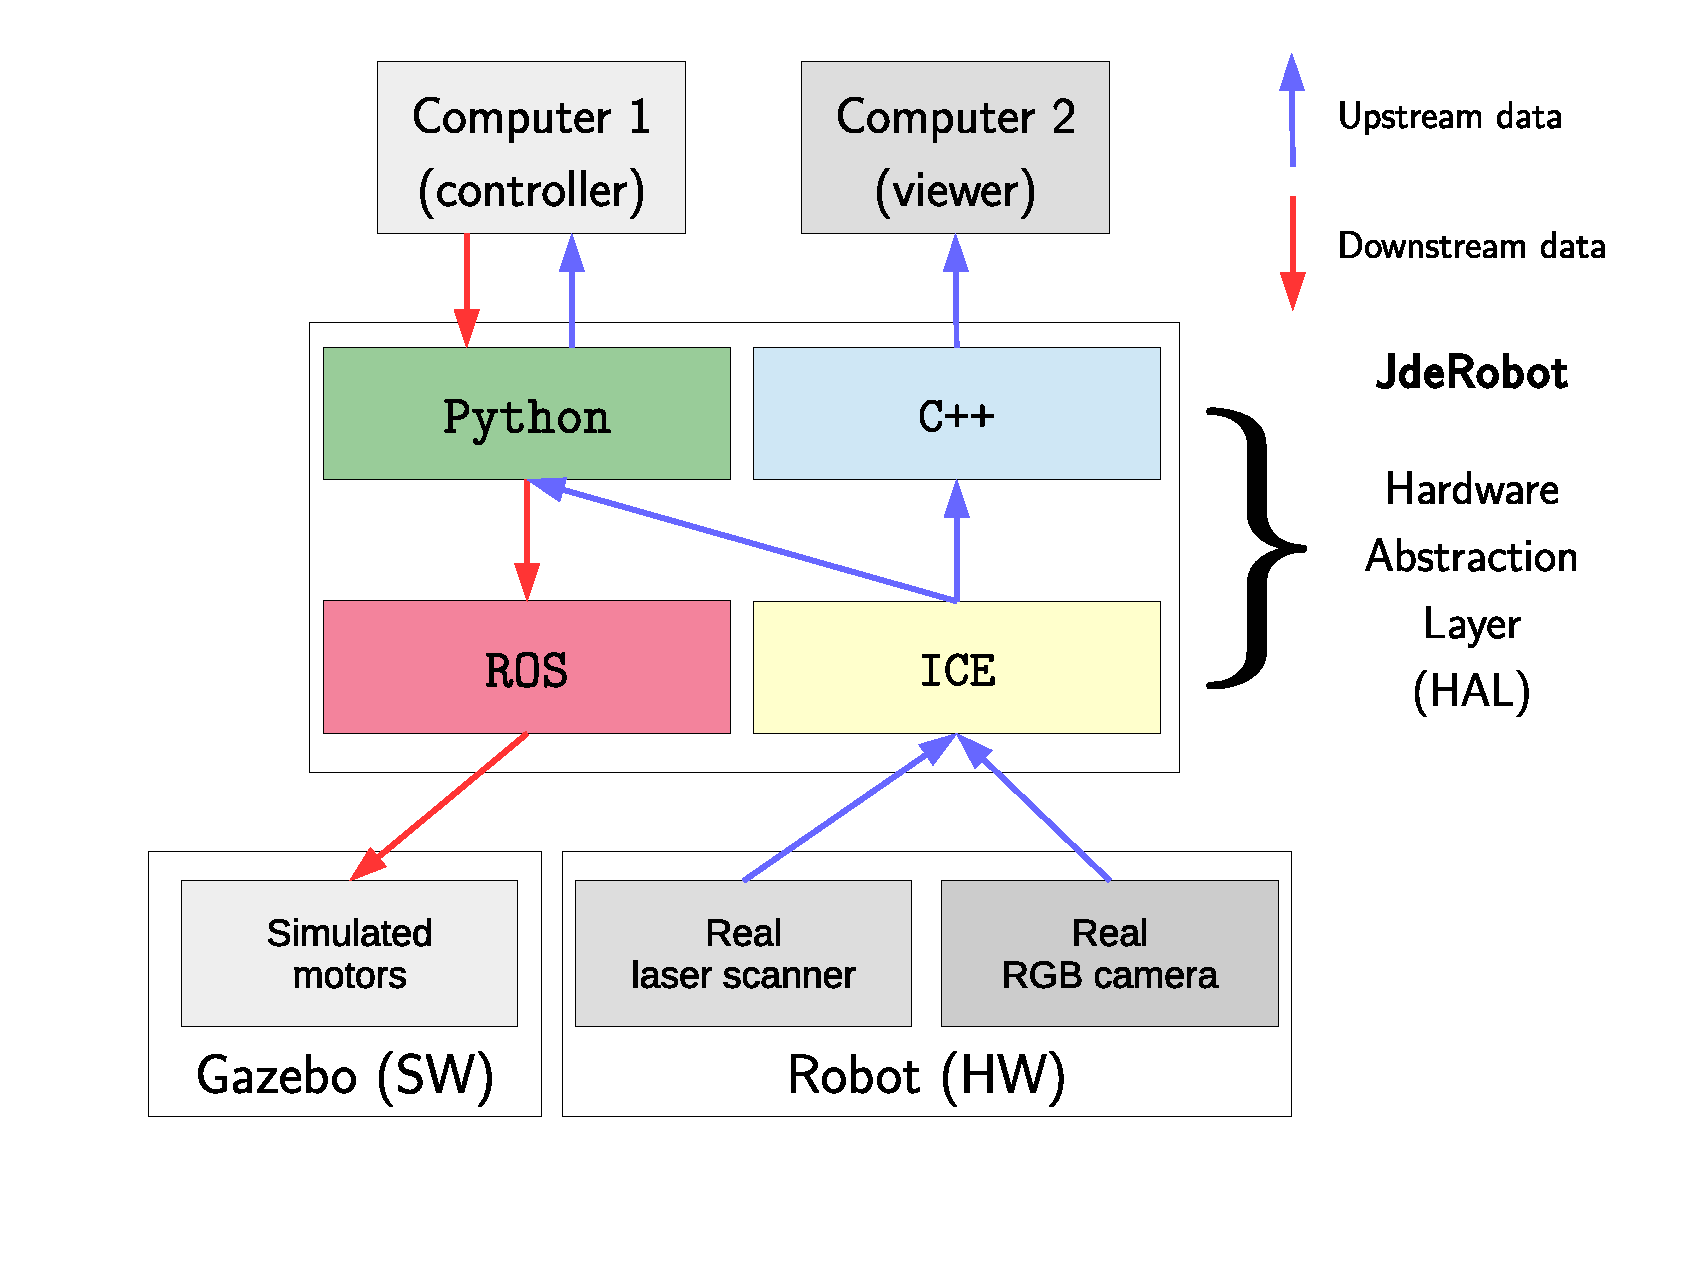
\includegraphics[width=4in]{images/jderobot_hal}
			\caption{JdeRobot abstraction layer, and a possible use distributed, multi-middleware scenario.}
			\label{fig:3_jderobot_hal}
		\end{figure}
		
.
		
		\item \textit{Wide device support:} JdeRobot provides full compatibility with ROS Kinetic Kame, so it can perfectly integrate ROS Nodes (in our concern, we can communicate with the Turtlebot and the Xtion devices via several topics that the ROS intermediate nodes open).
		
		\item \textit{Threaded software architecture for robotics applications:} as it is introduced at  \cite{jmplaza-phd}, inside a component, we will find one or more threads. These threads run concurrently with an specific timing (so it does not overload the CPU in vain if a few iterations per second are enough for a vivacious and correct response).\\
		
		These schemes perform different tasks each, on a non-blocking way, and share memory. This has been followed on a comfortable way on our implementation: the threads are independent, but the tasks they control are performed by Python objects, which are interconnected between them:
		
		
	\end{itemize}
	
	Now, in the next subsections, we will examine which of the available JdeRobot components, apart of the infrastructure, have been of greatest interest for us.
	
	\subsection{Digit Classifier node}
	\label{sec:3_digitclassifier_jderobot}
		This JdeRobot component was originally designed by David Pascual \cite{dpascualhe} and Nuria Oyaga \cite{noyaga}, and it was used on this project to land on the field of neural networks.\\
		\begin{figure}[h]
			\centering
			\includegraphics[width=4in]{images/digitclassifier}
			\caption{\texttt{DigitClassifier} on action.}
			\label{fig:3_digitclassifier}
		\end{figure}
		
		
		In rough outline, its function is to classify on-demand or in real-time the incoming images from a video source, mapping them into digits from $0$ to $9$. There are two identical version, differentiated on the underlying framework (Keras or Caffe). On \autoref{fig:3_digitclassifier} we can see its operation: it processes an image extracting the shown digit and showing the class that the network has assigned to it.\\
	
	
	\subsection{evicam\_driver driver}
	\label{sec:3_evicam_driver}
	This driver, bundled into JdeRobot\footnote{\url{https://github.com/JdeRobot/JdeRobot/tree/master/src/drivers/evicam\_driver}}, allows the user to send movements commands to a Sony EVI D100P camera \autoref{fig:3_evi}) and to retrieve information from it, creating an ICE endpoint that is ready to interact with the camera \emph{PT} (Pan, Tilt) motors.\\
	
	As this is a low-level driver, written in C++, it requires to be used on a specific way, which has been documented\footnote{\url{https://jderobot.org/Handbook\#PanTilt_Teleop}} to be easily applied in the future. This driver defines an interaction API with the camera, which allows us to get the values from the  encoders:
	\begin{lstlisting}
import config
import comm
...

cfg = config.load('yml_configuration_file')
jdrc = comm.init(cfg, 'NodeName')


# Instantiation for the motors:
PTMotors = jdrc.getPTMotorsClient('NodeName.PTMotorsEndpoint')

print(PTMotors.getLimits()) # Shows the max/min values for pan, tilt 
                            # and each speed.

print(PTMotors.motors.data) # Shows the current values for pan, tilt
                            # and each speed.

# Let's move the camera! As easy as:
PTMotors.setPTMotorsData(new_pan, new_tilt, max_pan_speed, max_tilt_speed)
	\end{lstlisting}
	
	\subsection{comm library}
		\label{sec:3_comm}
		\texttt{comm} is the basic library included on JdeRobot to perform communications between different components. It supports all the data flows in a typical scenario (\autoref{fig:3_jderobot_hal}).\\
		
		\texttt{comm} consists on a collection of bindings to easily create a link between two components, or between a device and a component. On the lowest level, we can use it relying on ROS (through topics as it was explained before on \autoref{sec:3_ros}), or through an ICE proxy. ICE\footnote{\url{https://zeroc.com/products/ice}} is an object-oriented middleware that, in our purpose, allows to abstract a data flow to a TCP/IP endpoint (an address/hostname, and a port), which can even support a communication between two or more programs inside the same machine.\\
		
		To create a communicator with \texttt{comm}, it needs the specification for that link (underlying middleware, topic/endpoint, etc.), so it uses the JdeRobot standard: YML\footnote{Legible data serialization format.} configuration files, which must follow a similar format to  \autoref{fig:3_yml_format}.
		\begin{figure}[h]
			\centering
			\includegraphics[width=4in]{images/yml_format}
			\caption{YML format required by \texttt{comm}.}
			\label{fig:3_yml_format}
		\end{figure}
		
		In the previous example (\ref{sec:3_evicam_driver}) we can see an example of an instantiation of a global communicator through \texttt{comm} (which then provides the clients to interact with the device).
		
\section{OpenCV library}
	OpenCV (\emph{Open Source Computer Vision}) is a C++/Python/Java open-source library\footnote{\url{https://opencv.org/}} (natively written in C++) for Computer Vision purposes. Among the classic/\emph{state-of-the-art} methods it bundles, we can find functions suitable for face recognition, image stitching, eye movements following, establishing markers for augmented reality, etc.\\
	
	Its general focus is \emph{efficiency and real-time functionality}, thank to low-level optimizations on the system hardware (i.e. integration with Nvidia CUDA and OpenCL GPU processing libraries). Thus, the excellent performance achieved by this open source library has turned it into the \emph{de facto} standard between every kind of users (from researchers to big companies or even governmental bodies, as their website stands).\\
	
	The main benefit we have grabbed from this library (on its version 3.3.1) has been mainly for image analysis (such as \emph{Haar Cascade} classifiers, or edge detectors) or transformations (color conversions, gaussian blurrings, etc.).\\

\section{NumPy library}
	NumPy\footnote{\url{http://www.numpy.org/}} (\emph{Numeric Python}) is a library for Python (written in C++), born to extend the numerical abilities of this language. It provides a powerful \texttt{array} class, which allows to keep a N-dimensional collection of values/objects in a really handy way (in comparison with Python's standard \emph{lists}). It also provides a rich interface to describe the arrays (such as advanced indexing, shaping, data formatting, etc.).\\
	This will such an useful resource on this work, for 3 main reasons:
	\begin{itemize}
		\item \emph{Matricial representation of images:} every processed image is handled as matrices or bigger order tensors (the concept of matrix generalized for any number of dimensions), so visualizing/slicing them becomes a trivial task.
		\item \emph{Abstract structure to keep objects:} it allows to store different objects in a \texttt{np.array} object, providing an advanced API for indexing, and conditional checks to instantly retrieve the elements fulfilling a specific condition.
		\item \emph{Saving variables into disk:} this is an useful feature for debugging purposes. \texttt{np.save()} allows to save any variable (even non-NumPy ones, like dictionaries), finding it on a \texttt{.npy} file, ready to be traced and debugged.
	\end{itemize}

In the same way than OpenCV, this is a numerical library widely adopted between Python users. This is due to the easiness of handling of its types and structures, that provides an immediate data exchange format with other parties software. It has made of it our main numerical engine on the developed purposes, having used it on its version 1.14.5.



\section{TensorFlow framework}
	\label{sec:3_tensorflow}
	TensorFlow\footnote{\url{https://www.tensorflow.org/}}, which has been the core component of this project, is an open-source software framework for high performance numerical computation. It was originally created by the Google Brain team, and it offers an excellent background for \emph{machine learning} tasks.\\
	
	Its internal functionality is based on \emph{graphs}, composed by nodes which operate and exchange data values establishing \emph{a flow of tensors} (as previously described, a tensor is the general term to describe a multidimensional structure). These tensors are handled in the backend of TensorFlow, so performing operations with tensors is really fast, in comparison with high-level mathematical libraries (NumPy). A tensor can be formed of different data types (images, words, poses, numbers, etc.), which is the key for the versatility it offers for a large variety of projects\footnote{\url{https://github.com/jtoy/awesome-tensorflow}}.\\
	
	\begin{figure}[h]
		\centering
		\includegraphics[width=4in]{images/tf_graph}
		\caption{Basic graph on TensorFlow (2 convolutional layers fed to a cost function).}
		\label{fig:3_tf_graph}
	\end{figure}
	
	All these possibilities make TensorFlow a very optimized ecosystem to implement \emph{deep learning} models (Deep Neural Networks). In addition, it is optimized for parallel GPU hardware. This gives a network the opportunity to experiment a performance boost, since it can reduce significantly the time it takes to make an inference (and even work on a system with a cluster of GPUs, although this is focused to more exigent systems than the one we create on this work). For our\\
	
	Since it was launched (November 2015), it has been adopted by many big companies which have used TensorFlow as the base for their Artificial Intelligence applications, such as Twitter, Intel, Google, eBay, Xiaomi, Nvidia, etc.\\
	
	As we will see later in the specific components, it allows to \emph{train} a neural network (for its later use) or even \emph{load} a specific model (kept on a Google Protobuf\footnote{Google's open source mechanism to serialize structured data.} \texttt{.pb} file). This is a really interesting feature, given that we are able to retrieve a bunch of pretrained models and embed them into a generic neural network.\\
	
	The version we have been using along the project is the last available one nowadays (1.9.0), compiled from sources on a Nvidia GPU (through CUDA on its 9.2.88 version), in order to squeeze the maximum inference speed possible.\\
	
	We have also also taken advantage of an included tool, \emph{TensorBoard}, which allows to \emph{visualize} interesting contents about a neural network, from a log trace of its execution. It is possible to visualize the \emph{graph} (including nodes, tensor shapes, operations, etc.). Also, it provides a functionality to analyze the obtained weights for each layer, on advanced analysis techniques, as PCA (\emph{Principal Component Analysis}). We have used it to visualize all the networks we design or import.




\section{Keras framework}
	As it is stated in \cite{dpascualhe}, Keras is a high-level \emph{neural network framework}, written in Python and capable of running on top of either TensorFlow or Theano (another \emph{deep learning} library).\\
	
	Hence, it is an abstraction with the goal of programming and handling a neural network on an simpler way, relying on a powerful library (treated as \emph{backend}) as TensorFlow to perform all the numeric operations. As well as TensorFlow, it is capable of loading previously compiled and saved models, on the serialization standard HDF5\footnote{Hierarchical Data Format (v.5): general purpose format to store and manage data.} (\texttt{.h5} files).\\
	
	In our project, support has been provided to use this framework (selecting it on the YML configuration file) on its version 2.2.0, although our main interest has been TensorFlow due to the significative difference of processing speed between both frameworks (being TensorFlow twice as fast as Keras).
\section{PyQt framework}
	Qt\footnote{\url{https://www.qt.io/}} is an cross-platform object-oriented framework for building GUIs (\emph{Graphical User Interfaces}), originally developed by a Nokia department. It is distributed under a commercial license, although it has a standard GPL license for open-source projects.\\
	
	A third party company (RiverBank Computing) developed PyQt, a set of Python bindings to interact with Qt (originally written in C++). It is structured in units called \emph{Widgets}, which contain blocks (\emph{Labels}).\\
	
	All this allows to easily deploy a GUI-based(\emph{Graphic User Interface}) program:
	\begin{figure}[h]
		\centering
		\begin{subfigure}[h]{0.55\linewidth}
			\centering
			\begin{lstlisting}
import sys
from PyQt5 import QtGui, QtWidgets

def window():
	app = QtWidgets.QApplication(sys.argv)
	w = QtWidgets.QWidget()
	b = QtWidgets.QLabel(w)
	b.setText("Hello World!")
	w.setGeometry(100,100,200,50)
	b.move(50,20)
	w.setWindowTitle("PyQt")
	w.show()
	sys.exit(app.exec_())

if __name__ == '__main__':
	window()
			\end{lstlisting}
			\caption{\emph{Hello world} example code.}
		\end{subfigure}
		\qquad
		\begin{subfigure}[h]{0.35\linewidth}
			\centering
			\includegraphics[width=3in]{images/pyqt_helloworld}
			\caption{Resulting window.}
		\end{subfigure}
		\caption{Example of a \emph{Hello World} window with PyQt5 bindings.}
		\label{fig:3_pyqt_helloworld}
	\end{figure}
	
	As it is the last available version at the time this is developed, we have used the version 5 of Qt. Hence, our binding library is \texttt{PyQt5}, which has been used to build a live-capable GUI on an intuitive way, in all the developed tools.\\
	
\section{threading library}
	\label{sec:3_threading}
	\texttt{Threading}\footnote{\url{https://docs.python.org/2/library/threading.html}} is a Python standard library which offer a high-level API for threading processes. This means to run programs on more than one single job for the CPU, which allows to be capable of perform several tasks on a simultaneous way.\\
	
	This is very convenient for our purpose, as we want to stick to a multiprocessing paradigm. So, this way we can have dedicated threads to grab the new camera images, update the GUI, and make the Neural Network to load new inferences on the last image detected.\\
	
	The \texttt{threading} provides a generic class for a thread. Our only task is to create a custom class which inherits it, customizing the \texttt{\_\_init\_\_} and \texttt{run()} methods our own way:
	

	\begin{lstlisting}
...
import threading
from datetime import datetime
...

class MyThread(threading.Thread):

	def __init__(self, foo, bar):
		'''
		This is the method which will be called at the creation of the thread.
		'''
		self.my_foo = foo
		self.my_bar = bar
		self.time_cycle = 100 # ms
		threading.Thread.__init__(self)  # Rest of the initialization.
		
		
	def run(self):
		'''
		This is the task the thread will perform once.
		If we put an infinite loop inside, we have a periodic thread.
		'''
		while True:
			start_time = datetime.now()
			# Grab an image, or run an inference on the neural network...
			self.my_foo.doMyStuff(self.my_bar)
			end_time = datetime.now()
			dt = end_time - start_time
			
			# If it did not take the refresh time, it sleeps until it arrives.
			if dt < self.t_cycle:
				sleep(self.t_cycle - dt)
				
	\end{lstlisting}
	
In addition, as we can see, it is possible to control the update period of the thread, so we can decide how much time it will be elapsed between two consecutive executions of the thread task (and of course this is a tunable parameter).\\

The version we have used is the standard one included with the Python installation.


% ---- Perception module ----
\section{Perception Module}

This module is responsible for apprehending the incoming images (RGB and depth) from the sensor, and generate a significant output to be interpreted by the actuation module. Its structure follows a certain pipeline with four steps: person detection, face detection, person and face trackers, and face reidentification. This pipeline allows the system to discern if the target person is being seen right now. 

\subsection{Person Detection}

First, the incoming RGB images are passed through an \emph{object detection} module. It is powered by a pretrained CNN, which has a special architecture designed in \cite{ssd} for this purpose: SSD (\emph{Single-Shot Multibox Detector}). This detection model type stands out by its prediction speed, because \emph{it performs a single feed-forward pass} of the image through the network, unlike other state-of-the-art techniques. These other approaches perform successive feed-forward passes through the network, what makes them consequently much slower. Before choosing SSD for the proposed system, several detection architectures were compared and their corresponding typical inference times were measured (Table \ref{tab:model_tests}).

\begin{table}[h]
	\centering
	\begin{tabular}{|c|c|c|c|}
		\hline
		\textbf{Architecture} & \textbf{Base network} & \textbf{Dataset} & \textbf{Mean inference time} (ms) \\ \hline
		ResNet  & Inception  & COCO & 820.71 \\ \hline
		SSD  & MobileNet  & COCO & 107.43 \\ \hline
		ResNet  & 101  & COCO & 786.49 \\ \hline
		ResNet  & 50  & COCO & 515.28 \\ \hline
		ResNet  & 101  & COCO & 63.97 \\ \hline
		Faster-RCNN  & ImageNet  & ILSVRC2014 & 703.99 \\ \hline
		Faster-RCNN  & Inception  & COCO & 352.20 \\ \hline
		ResNet  & 50  & COCO & 793.87 \\ \hline
		SSD  & MobileNet  & COCO & 102.85 \\ \hline
		ResNet  & 101  & COCO & 898.59 \\ \hline
		Inception  & ResNet  & OID & 792.42 \\ \hline
		\textbf{SSD Lite}  & \textbf{MobileNet}  & \textbf{COCO} & \textbf{68.13} \\ \hline
		ResNet  & 101  & Kitti & 111.29 \\ \hline
		Inception  & ResNet  & OID & 667.76 \\ \hline
	\end{tabular}
	\caption{Timing performance tests for several detection models. The selected implementation is SSD Lite.}
	\label{tab:model_tests}
\end{table}

On this module, the desired image to input has to be reshaped to 300$\times$300 px, which is a typical shape for this type of CNN architecture. As shown on Fig. \ref{fig:perception_ssd}, it extracts a set of activation maps on its \emph{base network} o Feature Extractor (\emph{MobileNet}) in the selected network model, and position and class inferences are made later, on multiple image scales. Finally, a \emph{Non Maximum Suppressor} is applied, retaining only the most confident detections, which are adjusted to a correct bounding box shape.

\begin{figure}[h]
	\centering
	\includegraphics[width=10cm]{images/SSD_schematic}
	\caption{Schema of the SSD architecture.}
	\label{fig:perception_ssd}
\end{figure}


This network provides an accurate and efficient object detection, returning for each processed image:
\begin{itemize}
	\item \emph{Classes:} the detected classes (person, cell phone, airplane, dog \dots) inferred for each detected object.
	\item \emph{Scores:} the confidence $\in [0,1]$ the network has on each object belonging to the estimated class.
	\item \emph{Boxes:} the coordinates of the rectangular \emph{bounding box} which wraps the detected object, expressed as the coordinates of two opposite corners of it.
\end{itemize}

Although the used SSD model is capable to detect up to 80 object classes, the proposed system only retains those detection corresponding to \emph{persons}, as it is what we are interested to follow. All this results on a light \emph{person detection}, perfectly capable to work on a real-time operation on a regular computer. 

In addition, our implementation is capable to handle different network models and architectures on a \emph{plug and play} way, just pointing the model file (in the specific TensorFlow \texttt{.pb} format) in the configuration file of the program.


\subsection{Face detection}

Once the existing persons on the image have been detected, the next step is to search their faces, in order to know whether any of them corresponds to the target person to follow. For this the classical Viola and Jones face detection algorithm \cite{viola-jones} has been used. This algorithm, which comprises \emph{Haar} features (Fig. \ref{fig:perception_haar}), is a simple algebraic method which takes advantage of the typical illumination pattern of a face (due to its physical shape) to detect promising regions of the input image to contain a face. To test a \emph{Haar} feature on a specific grayscale image, the feature is slided through it, and a simple operation is performed (black pixels subtracted to white ones). If the result is positive along all the feature, the region where it has been applied passes the test.


As the previous block detected persons inside the image, this face detection algorithm is only applied inside the instance of the detected persons, in order to speed up the system and avoid false positive detections. Each of detected person is divided into \emph{regions}, which are passed through a \emph{cascade} of tests, where the non-compliant regions are immediately discarded. The accepted ones pass to a slightly more complex feature each time, and the regions which pass all the features are supposed to contain a face. This progressive region dismiss makes it an efficient algorithm, capable of run simultaneously with the rest of processes. This entire process is performed with an OpenCV function \footnote{Open source image processing library.}.

\begin{figure}[h]
	\centering
	\includegraphics[width=8cm]{images/haar_on_face}
	\caption{\emph{Haar} features applied on a face.}
	\label{fig:perception_haar}
\end{figure}


\subsection{Person and face trackers}

The two previous steps detect persons and faces, but although they behave in a robust way their outputs can suffer spurious false negative or false positive detections, due to lighting or occlusions. As they can interfere with the desired following capability, the third step palliates their effect implementing time-spatial \emph{trackers}, which filter the detection outputs (\emph{candidate detections}). The tracker associates to each person/face its coordinates inside the image, and takes into account the number of successive frames on which it has been detected. If it surpasses a \emph{patience} threshold, it is considered a reliable (\emph{tracked detection}). Otherwise, it is taken as a spurious output and ignored. In addition, each \emph{tracked detection} is remembered for some frames even without new fresh detections. This way, a partial occlusion of a particular person does not cause the elimination of that person, until it has not been lost for a while.
% The same happens with void detections which generally happen on a punctual way on a frame.

This tracking step can be observed in Fig. \ref{fig:perception_tracker}, in the \emph{person detection} case, but it is applied in the same way for \emph{face detection} in the proposed system. In addition, it is not necessary to detect the person face every time, as the person tracker is capable to infer that a new person detection on a near location to the last position of the target person corresponds to the new location of the tracked person, without needing to see again her face.

\begin{figure}[h]
	\centering
	\includegraphics[width=12cm]{images/person_tracker}
	\caption{Tracking process for a person detection.}
	\label{fig:perception_tracker}
\end{figure}


\subsection{Face reidentification}

The previous trackers turn the spurious output of the detection systems into tracked and reliable detections. Hence, they can be used to perform \emph{identification} tasks. For this purpose, a parallel CNN is used, the \emph{FaceNet} \cite{facenet}. This network \emph{maps} a face image, extracting some key features, into a 128-dimensional Euclidean space, where faces are represented by what is called \emph{embeddings} (feature vectors). The Euclidean $L^2$ distance (Eq. \ref{eqn:eucl_distance}) existing between two of this embeddings stands for the \emph{face similarity} between that faces. Hence, we can consider that two embeddings belong to the same face if their distance is below a threshold, which has experimentally been set to $1.1$.

\begin{equation}
d(\vec{f_1}, \vec{f_2}) = \sqrt{\sum_{i=1}^{128}(f_{1_i} - f_{2_i})^2}
\label{eqn:eucl_distance}
\end{equation}

The proposed solution makes use of this, computing on real time the embeddings of each detected (and tracked) face. Once this has been performed, it compares the similarity between these embeddings and the one corresponding to the target person. The target person embedding is computed when the program starts, from a given image file of the \emph{person to be followed}.

To avoid penalties on similarity due to lighting conditions, a previous blurring and \emph{prewhiten} (on Eq. \ref{eqn:perception_normalization}, with $x$ as the color channel, $\mu$ as its mean and $\sigma$ as its standard deviation) are performed on each face put on the \emph{FaceNet}.

\begin{equation}
x' = \frac{x - \mu}{\sigma}
\label{eqn:perception_normalization}
\end{equation}

In Figure \ref{fig:perception_distance} the same face is seen in different lighting situations, and all of them yield embeddings with a distance lower than the threshold.

\begin{figure}[h]
	\centering
	\includegraphics[width=10cm]{images/facenet_prewhiten}
	\caption{Relative distances between the same face on different lighting situations.}
        \label{fig:perception_distance}
% Color patterns on the right images are not representative, as they depend on the numeric range of the plotted image.}
\end{figure}







% ---- Actuation module ----
\section{Actuation module}

After the \emph{perception} tasks, the system has obtained the maximum possible certainty about the persons present in the current RGB image, as well as their condition of being or not being the one to be followed.\\

The next functional block, the \emph{actuation} one, is responsible of generating a suitable command to the robot motors, in order to move towards the followed person, in case it is being seen in the current frame. To do so, it follows its own pipeline, explained next.


\subsection{Following behavioral}

As it has been stated, the input for this element is the information yielded by the \emph{perception} block: the \emph{tracked persons} parameters (position, face, ``is or not the followed person"). From this information, the new \emph{actuation} block has to infer which attitude to take (depending on the state of the system on the last iteration). This is implemented with a \emph{case-based} behavioral, which follows the \emph{flow chart} represented on Fig. \ref{fig:actuation_flow}. It can be seen that the response depends on \emph{mom} (the semantical name given to the followed person), as it can be \emph{lost} or \emph{tracked and followed}.\\

\begin{figure}[h]
	\centering
	\includegraphics[width=2.5in]{images/flowchart}
	\caption{\emph{Flow chart} followed by the case-based behavioral, depending on the previous state.}
	\label{fig:actuation_flow}
\end{figure}

If the followed person is found among the tracked persons, the system follows it. It can observed as well that, as it was mentioned before, the system does not need a continuous face feedback to follow the target person, as it just needs to be still seen (that time-spatial continuity is provided by the previously described trackers). In addition, if a new face is found, and it satisfies the criteria of similarity with the reference face, the \emph{followed} role is swapped to that new person, which begins to be followed by the system.\\


\subsection{Error computation}

Once the system has recognized the target person into the image, in case it is being seen, it proceeds to an \emph{error computation}, in order to determine the strength of the required movement to move towards that person. As the robot used on the proposed system moves in two dimensions, we perform a dual error computation:

\begin{itemize}
	\item \emph{Angular error:} the most accurate position for the system with respect to the person is to be aligned with it. This way, the person appears right in the horizontal center of the image. Hence, we can compute the \emph{angular error} as the subtract of the center coordinates and the center of the person's bounding box, in the horizontal dimension. This process,  represented in Fig. \ref{fig:h_error}, will give a quantization of the necessary turn to be performed.\\
	
	\begin{figure}
		\centering
		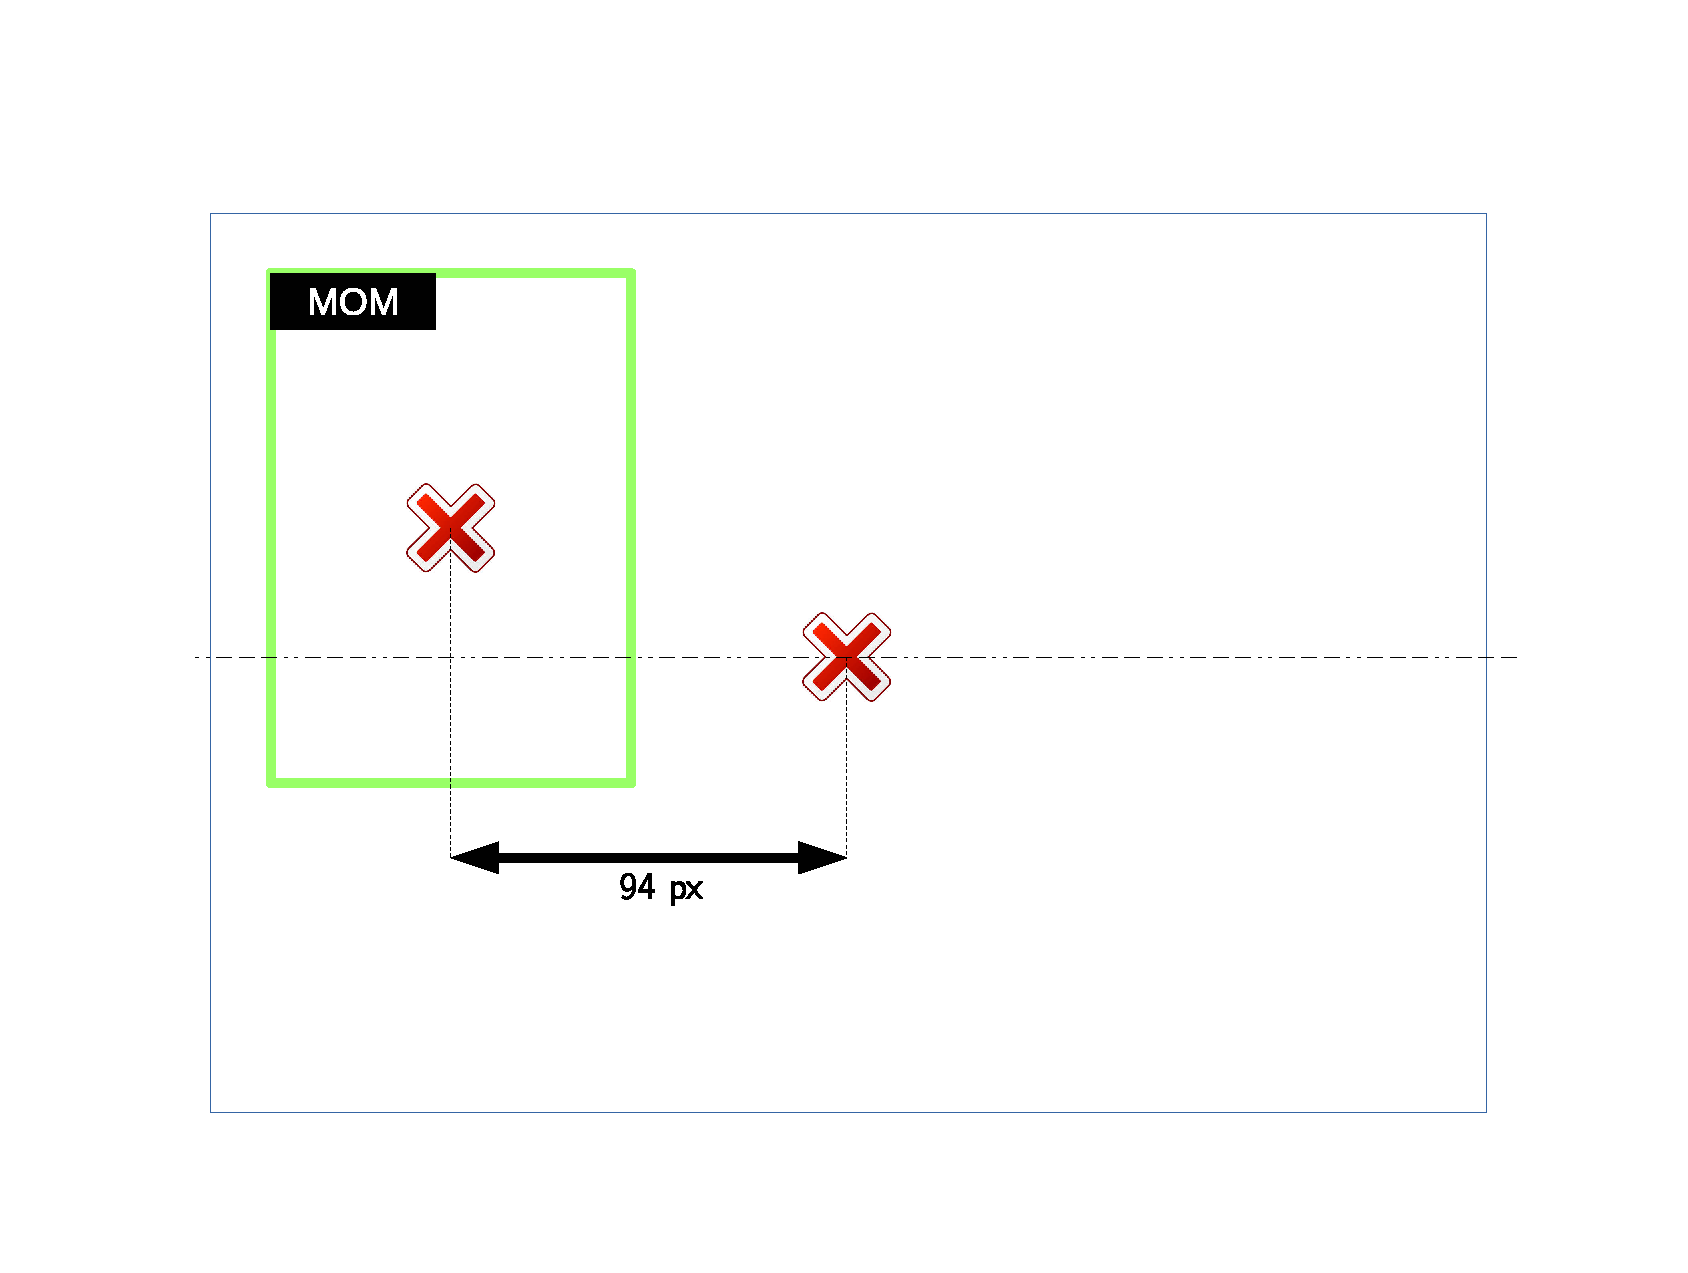
\includegraphics[width=2.4in]{images/h_error}
		\caption{Computation of the angular error between the system and the followed person.}
		\label{fig:h_error}
	\end{figure}
	
	
	\item \emph{Linear error}: as the implemented sensor is a RGBD camera, it will provide the system a \emph{depth} image. As it is aligned with the RGB image, the coordinates of the person inside the depth image are the same than the RGB ones. Hence, it allows to \emph{locate} the person inside the depth map.\\
	
	In consequence, a 10$\times$10 grid sampling of the depth values inside the person box (putting care on avoiding the margins, in order to measure only inside the person) allows to collect a serie of measured distances to the person. This system performs that process, and computes the \emph{median} of that set of measures, taking the result as the distance from the robot to the person, as seen on Fig. \ref{fig:v_error}.
	
	
	\begin{figure}[h]
		\centering
		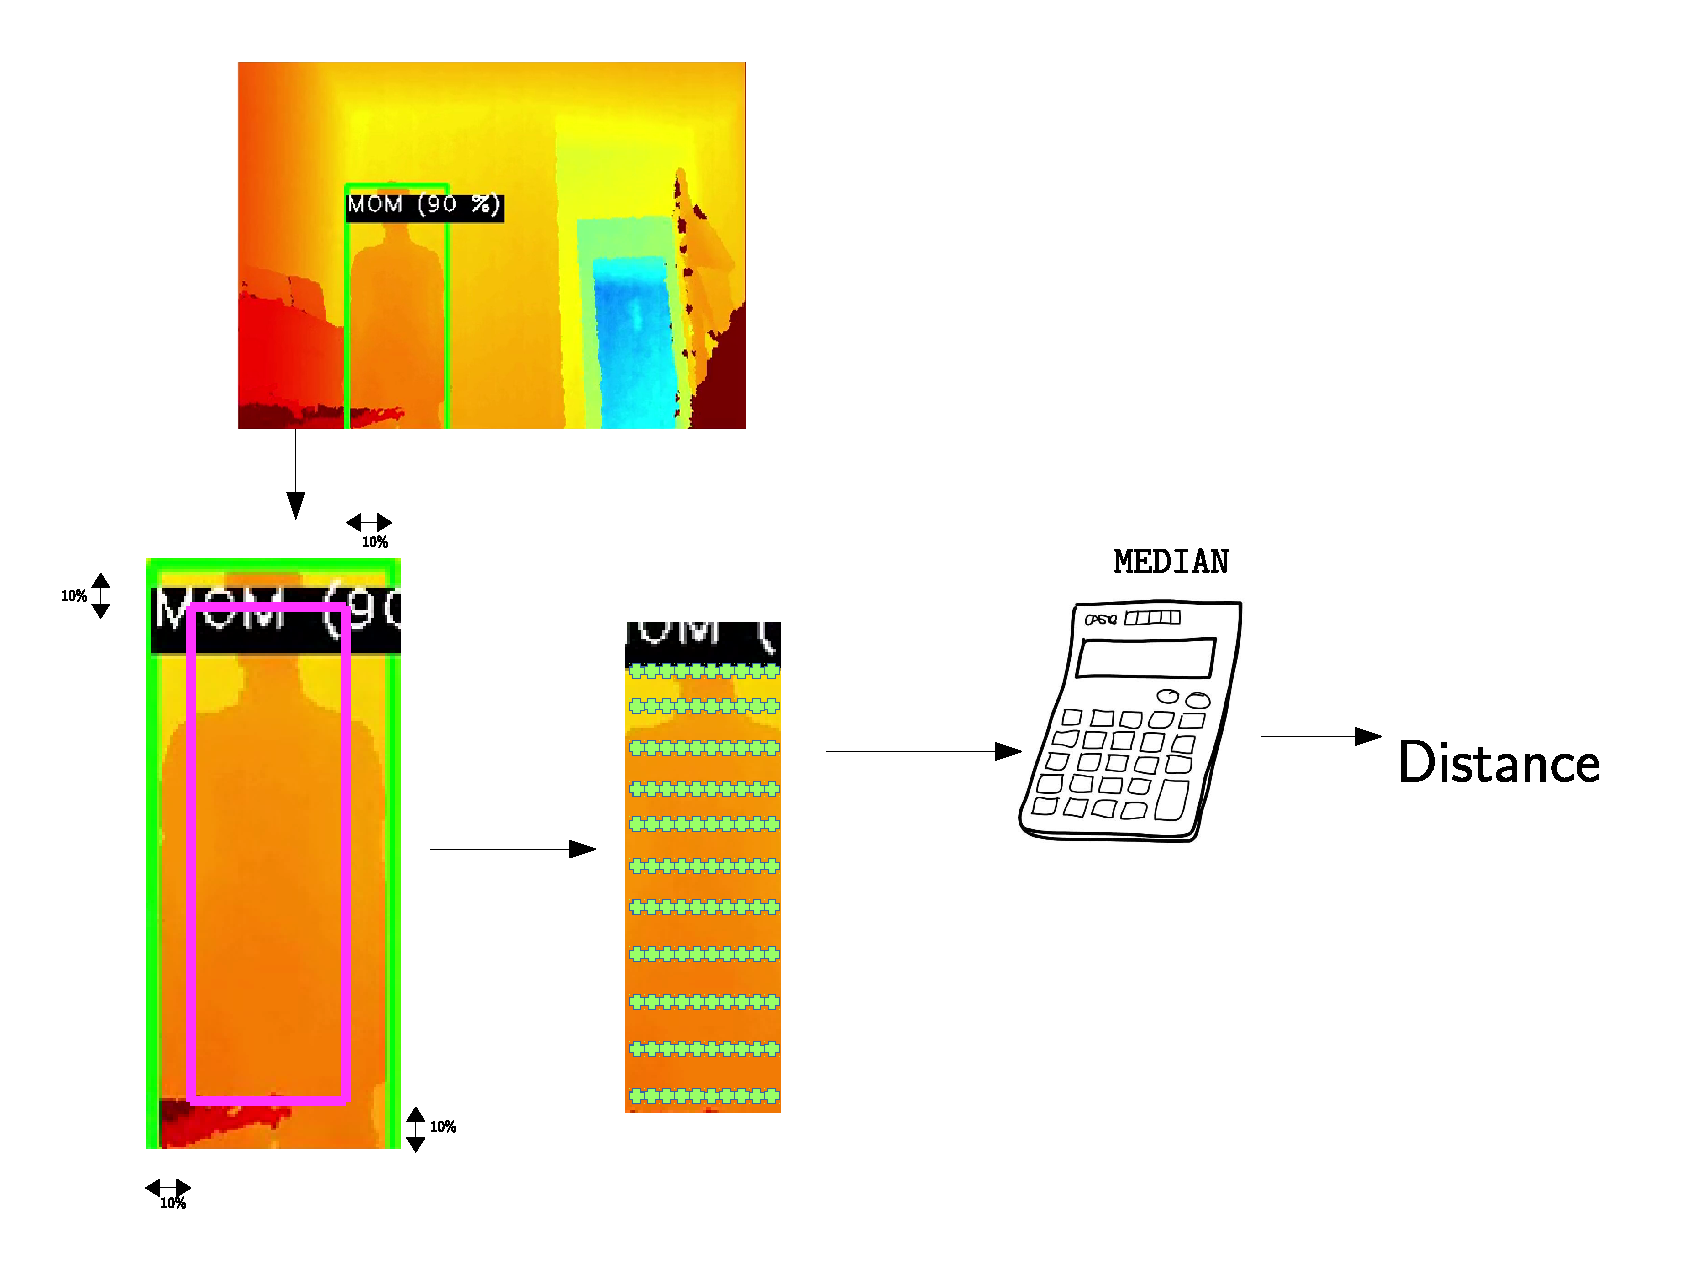
\includegraphics[width=2.5in]{images/distance_error}
		\caption{Computation of the linear error between the system and the followed person.}
		\label{fig:v_error}
	\end{figure}
	
\end{itemize}


So far, the system is capable to determine a numerical error value to measure the magnitude of the required response.\\


\subsection{Movement response}

The previous measures are required to determine the \emph{relative position} of the robot and the target person. It is used as an input to compute the most suitable response.\\

As the system is not designed to move literally to the position of the person, but to just maintain a following behavior, a \emph{dead zone} is established in each dimension. These dead zones (illustrated on Fig. ) will cause the robot not to move anymore towards the person, as the person is considered \emph{under control} when it is placed inside.\\


\begin{figure}[h]
	\centering
	\includegraphics[width=2.5in]{images/dead_zones}
	\caption{Dead zones on each dimension, where the person is considered under control.}
	\label{fig:dead_zones}
\end{figure}


If the person is outside these dead zones, a physical response is required, with the purpose of \emph{carrying} that person inside the dead zone. For this action, each dimension implements a \emph{PID} controller, which establishes a \emph{closed-loop} feedback system, as described on \cite{pid-controller}. This allows to keep in mind previous responses, to achieve the optimum fitting in every iteration. This means, for example, to accelerate if the person is not going any closer, or to step hard on the brake if the person suddenly gets too close.\\

The implemented \emph{PID} controllers (an angular and a linear one) have been experimentally tuned to obtain the most suitable parameters for our operation, obtaining the values in Table \ref{tab:pids}.\\

\begin{table}[h]
	\centering
	\begin{tabular}{|c|c|c|}
		\hline
		\textbf{} & \textbf{Linear} & \textbf{Angular} \\ \hline
		$k_p$     & 2               & 7                \\ \hline
		$k_d$     & 0.1             & 0.5              \\ \hline
		$k_i$     & 3               & 10               \\ \hline
	\end{tabular}
	\caption{Optimal found values for the parameters in each PID controller.}
	\label{tab:pids}
\end{table}

This way, the system can output a speed value with a tight adjustment to the values required by the situation of the current iteration. The response obtained from this value is a \emph{reactive} one. This means that each value results in a new movement command, avoiding to perform movements longer than one iteration. For softness sake, what is sent to the motors is not this value, but the \emph{mean} between it and the last sent one. This way, it results on a slightly longer convergence that helps to remove sudden movements.





\vspace{1.5in}

The previously described pipeline is executed \emph{once} per thread iteration, maintaining on concurrent threads each one of the two blocks (\emph{perceptive} one and \emph{actuative} one). This results on a new speed command to each one of the two available motors (angular and linear advances) on each iteration.

% ---- Experiments ----
\begin{figure}[h!]
	\centering
	\includegraphics[width=8cm]{images/exp_set}
	\caption{Robot used for the validation experiments.}
	\label{fig:exp_set}
\end{figure}


\section{Experiments}
\label{sec:experiments}

The developed system has been experimentally validated on a real robot and an indoor scenario. The TurtleBot-2 robot was used on the experiments, including an Asus Xtion Pro Live RGBD sensor. The onboard computer was a regular laptop, equipped with an Intel i5-4210U CPU, a DDR3 RAM of 8GB and a Nvidia 940M GPU (Figure \ref{fig:exp_set}). On this hardware resources (using GPU parallelization to run the neural networks, and choosing a lightweight \textit{SSD Lite }model), we achieved a stable detection rate of 14 fps, fairly enough to guide the robot on a seamless way. 

% \begin{figure}[h]
% 	\centering
% 	\includegraphics[width=4.5cm]{images/light_ko_2}
% 	\caption{Harsh lighting conditions.}
% 	\label{fig:exp_lighting}
% \end{figure}


The person detection and reidentification process can be observed on Fig. \ref{fig:exp_figures}. The system is succesfully able to re-identify the target person (\textit{mom}), even in challenging lightning conditions like in Figure \ref{fig:exp_figures}.

\begin{figure}[h!]
	\centering
	\includegraphics[width=12cm]{images/exp_tracking}
	\caption{Detection and face re-identification of the target person.}
	\label{fig:exp_figures}
\end{figure}

The complete system results show a robot finely following a particular person, even when that person does not face towards the robot. The behavior is fluent, with a refresh rate of 10 movements per second (as the SSD CNN is the lightest possible model, as seen on Table \ref{tab:model_tests}). This agility of the neural network for people detection helped substantially to minimize the time bottleneck. The following behavior can be observed on Fig. \ref{fig:exp_following}. Several videos of a typical execution are also publicly available \footnote{Full video test available on \url{https://www.youtube.com/watch?v=oKMR_QCT7EE}}.

\begin{figure}[h!]
	\centering
%        \includegraphics[width=12cm]{images/followperson_working.png}
	\includegraphics[width=12cm]{images/followperson_working2.png}
	\caption{Following behavior.}
	\label{fig:exp_following}
\end{figure}

% ---- Conclusions ----
\chapter{Conclusions}
\section{Conclusions}
	This final chapter will be destined to revisit the initially proposed objectives (\autoref{chap:2_objectives}). With a complete coverage of the performed tasks, as it has been described on the previous pages, we can contrast what has been achieved on each one of these objectives.\\
	
	\begin{description}
		\item[Classification] \hfill
			\vspace{0.2in} \\
			The first objective required to upgrade the scope for an existing JdeRobot component, \texttt{DigitClassifier}, designed to perform \emph{classification} tasks using \emph{deep learning} techniques.\\
			
			Its functionality was emulated using the \emph{deep learning} framework TensorFlow (core of this project), obtaining satisfactory results on the real-time digit classification task, training an \emph{in-house} neural network on our own, and obtaining initial knowledge about the framework and enough deep learning skills to move forward to more complex tasks.\\
			
			In light of the excellent achieved performance, the brand new TensorFlow implementation and the previous one (made with the Keras framework) were merged into an \emph{official JdeRobot} component\footnote{\url{https://github.com/JdeRobot/dl-digitclassifier}}, capable of commuting between both frameworks.
		
		\item[Detection] \hfill
			\vspace{0.2in} \\		
			After having accomplished a basic domain on \emph{deep learning} with \emph{classification} tasks, we tackled a more ambitious milestone: \emph{detecting objects on a real-time operation} (where there was no previous reference in the JdeRobot environment).\\
			
			Although the process of training a detection network was ruled out of the scope of the project (because of computational issues, as stated previously), we addressed the detection task using publicly available \emph{pretrained networks}. So, we developed a wrapping TensorFlow environment to \emph{abstract} the model (architecture, dataset on which it was trained, output format, etc.), and moved the neural network processing to a \emph{GPU environment} (to achieve the optimum refresh rate for a real-time operation).\\
			
			This remarkably efficient detection framework was demonstrated to be capable of real-time processing, so we have developed an entire node, \texttt{ObjectDetector}, to visually perform this task on an \emph{incoming image stream} (abstracting the source).\\
			
			Hence, the final result  has been a node displaying the bare current image, and aside the same one with the detected objects overlaid, indicating its location making use of a \emph{bounding box}, in addition to the decided \emph{class} the object belongs, and the \emph{score} (standing for the reliability level that prediction has).\\
			
			Once more, the excellent performance on real-time (using detectors with a SSD architecture under the shield) has driven us to integrate this node\footnote{\url{https://github.com/JdeRobot/dl-objectdetector}} in the JdeRobot environment as well, developing another package to do the same in Keras. This has enabled us again to be able to abstract the frameworks, and toggle one of them through the YML file. This component can be taken as a passage to \emph{alternative implementations} making use of the robust detection performance that \emph{deep learning} can yield (and not only drawing the results over the image). In addition, this has given us the capability of \emph{benchmarking} new models, as they can be transparently loaded into the created environment.
			
			
		\item[Tracking and following] \hfill
			\vspace{0.2in} \\
			The two previous milestones allowed us to accomplish \emph{state-of-the-art} purposes in the \emph{Computer Vision} field. As it has just been stated, \texttt{ObjectDetector} is a powerful tool to take advantage of a real-time detection system.\\
			
			So, as the final research objective, we have considered an \emph{actuation} system, which uses a powerful \emph{neural network} to accomplish an extra objective. In order to overlap our research with the prosperous field of \emph{robotics}, we have developed a component capable of \emph{following} a specific person (\emph{mom}). This has been achieved ringing into our set of tools concepts like a \emph{PID} controller, or behavioral schemes, which have throw in some extra knowledge.\\
			
			Additionally, this has demonstrated the possibility of finding \emph{synergies} between \emph{deep learning} and another kind of scientific fields, as it is currently made in tasks like processing sound, words, medical images, advertising, etc.
		
		\item[Personal fields] \hfill
			\vspace{0.2in} \\
			The previously described infrastructure we have created has allowed a novice investigator to check how important a \emph{correct coordination} is, when it is necessary dealing with tasks like a \emph{conjoint} development (as it had to be done at certain moments).\\
			
			In addition, a telecommunication engineer must know how to multiplex resources, even itself. The closest approach a human can achieve to this is \emph{TDMA}, so it's a key factor to be able to \emph{make a correct time assignment over incoming tasks}. This has allowed to learn the importance of keeping work tidiness and rigor, as well as a suitable level of \emph{compromise} (sustained through motivation to attainment), in order to be adaptive and be ready for a change of plans, or a readjustment of the requirements. All of these capacities make the difference between a long-term research project, and a simple homework task.\\
			
			On the other hand, in this kind of project it is important to keep a decent trace of the made work. This is essential in order to be able to go back in any moment, to revert some undesired effect, or just for consulting a past detail which we need to bring back. For this purpose, it has been very convenient to maintain the \emph{project's Wiki page}, for being able to have a glance on the achieved advances, and keep a trace of the temporal progress of the whole project.\\
			
			
			In the professional point of view, it has been essential to acquire further skills about \emph{version control systems}, as Git. If we take a look back, carrying through all the progress we made would have been no other thing than a hell. This can be an important benefit, as every development project in a corporate environment makes use of this kind of controls.
		
	\end{description}
\section{Future research lines}
	The proposed milestones on this project have been successfully achieved using a useful and innovative tool as \emph{deep learning}. Hence, it opens some interesting doors to future researches or improvements:
	
	\begin{itemize}
		\item \emph{Upgrade DigitClassifier:} for now, this component looks for the digit in a fixed window inside the image (the central square). Another module could be implemented to perform a \emph{character detection} in the image, using \emph{deep learning} as it is a really efficient implementation.
		
		\item \emph{Translate the nodes to a compiled language:} one of the main handicaps of Python is the fact that it is an interpreted language (much slower than a compiled one). So, a \emph{translation} to a lower level language as \texttt{C++} would be very interesting, as it is a widely supported language in this framework, and there are already very efficient \emph{deep learning} implementations on it (as \emph{Darknet/YOLO}).
		
		\item \emph{Use a deep learning face detector in FollowPerson:} the main advantage of the \emph{deep learning} systems is the robustness on the operation, so a facial detection system implemented with this technology could be a powerful resource to be able of performing a facial detection/validation in harshly lightened environments.
		
		\item \emph{Multimodal person detection/tracking:} some extra functionality could be squeezed of a RGBD sensor, like \emph{tracking a person in complete darkness}. As \emph{deep learning} systems offer good results distinguishing a person silhouette, we can perform people detection on a depth image (in fact, that is just what is being made in \autoref{fig:1_detectionsuite}).
		
		
		\item \emph{Add a navigation algorithm to FollowPerson:} the only movement commands sent to the Turtlebot are controlled by the relative position of the person with the robot. However, as the robot incorporates a laser sensor, we can add an \emph{obstacle avoidance} system, in order to perform a non-blind navigation towards the person.
	\end{itemize}









% ---- Bibliography ----
%
\begin{thebibliography}{6}
%

\bibitem{munoz2007people}
Mu{\~n}oz-Salinas, Rafael and Aguirre, Eugenio and Garc{\'\i}a-Silvente, Miguel.
People detection and tracking using stereo vision and color
\textit{Image and Vision Computing} 25(6), Elsevier, 2007.
% @article{munoz2007people,
%   title={People detection and tracking using stereo vision and color},
%   author={Mu{\~n}oz-Salinas, Rafael and Aguirre, Eugenio and Garc{\'\i}a-Silvente, Miguel},
%   journal={Image and Vision Computing},
%   volume={25},
%   number={6},
%   pages={995--1007},
%   year={2007},
%   publisher={Elsevier}
% }

% \bibitem{aguirre2014leg}
% Aguirre, Eugenio and Garcia-Silvente, Miguel and Plata, Javier.
% Leg detection and tracking for a mobile robot and based on a laser device, supervised learning and particle filtering
% \textit{ROBOT2013: First Iberian Robotics Conference}, Springer, 2014.
% @inproceedings{aguirre2014leg,
%   title={Leg detection and tracking for a mobile robot and based on a laser device, supervised learning and particle filtering},
%   author={Aguirre, Eugenio and Garcia-Silvente, Miguel and Plata, Javier},
%   booktitle={ROBOT2013: First Iberian Robotics Conference},
%   pages={433--440},
%   year={2014},
%   organization={Springer}
% }

\bibitem{aguirre2016multisensor}
Aguirre, Eugenio and Garc{\'\i}a-Silvente, Miguel and Pascual, Daniel,
A multisensor based approach using supervised learning and particle filtering for people detection and tracking,
\textit{Robot 2015: Second Iberian Robotics Conference}, Springer, 2016
% @inproceedings{aguirre2016multisensor,
%   title={A multisensor based approach using supervised learning and particle filtering for people detection and tracking},
%   author={Aguirre, Eugenio and Garc{\'\i}a-Silvente, Miguel and Pascual, Daniel},
%   booktitle={Robot 2015: Second Iberian Robotics Conference},
%   pages={645--657},
%   year={2016},
%   organization={Springer}
% }

\bibitem {rocapal2005}
%Calvo, R.: Comportamiento sigue persona con visión direccional, Proyecto Fin de Carrera, Universidad Rey Juan Carlos, 2004.
R.Calvo, J.M.Cañas, L.García-Pérez. 
Person following behavior generated with JDE schema hierarchy 
\textit{Poster in ICINCO 2nd Int. Conf. on Informatics in Control, Automation and Robotics}. Barcelona (Spain), sep 14-17, 2005. INSTICC Press, pp 463-466, 2005. ISBN: 972-8865-30-9

\bibitem {ssd}
Lui, W., Anguelov, D., Erhan, D., et al. 
SSD: Single-Shot Multibox Detector. 
\emph{CoRR}, abs/1512.02325, 2015.

\bibitem {viola-jones}
Viola, P., Jones, M. 
Rapid object detection using a boosted cascade of simple features. 
In \emph{Proceedings of the 2001 IEEE Computer Society Conference on Computer Vision and Pattern Recognition. CVPR 2001}, volume 1, pages I-511-I-518 vol.1, 2001.

\bibitem{facenet}
Schroff, F., Kalenichenko, D., Philbin, J. 
\emph{FaceNet}: A unified embedding for face recognition and clustering. 
\emph{CoRR}, abs/1503.038032, 2015.

\bibitem{pid-controller}
Åström, KJ., Murray, RM. 
\textit{Feedback Systems: An Introduction for Scientists and Engineers}, 2004.

\bibitem{xue2016tracking}
Xue, Hongyang and Liu, Yao and Cai, Deng and He, Xiaofei. 
Tracking people in RGBD videos using deep learning and motion clues. 
\textit{Neurocomputing} 204, pages 70-76, Elsevier, 2016. 
% @article{xue2016tracking,
%   title={Tracking people in RGBD videos using deep learning and motion clues},
%   author={Xue, Hongyang and Liu, Yao and Cai, Deng and He, Xiaofei},
%   journal={Neurocomputing},
%   volume={204},
%   pages={70--76},
%   year={2016},
%   publisher={Elsevier}
% }

\bibitem{koide2016identification}
Koide, Kenji and Miura, Jun.
Identification of a specific person using color, height, and gait features for a person following robot.
\textit{Robotics and Autonomous Systems} 84, pages 76-87, Elsevier, 2016.
% @article{koide2016identification,
%   title={Identification of a specific person using color, height, and gait features for a person following robot},
%   author={Koide, Kenji and Miura, Jun},
%   journal={Robotics and Autonomous Systems},
%   volume={84},
%   pages={76--87},
%   year={2016},
%   publisher={Elsevier}
% }

\bibitem{munaro2014feature}
Munaro, Matteo and Ghidoni, Stefano and Dizmen, Deniz Tartaro and Menegatti, Emanuele.
\textit{A feature-based approach to people re-identification using skeleton keypoints}.
2014 IEEE International Conference on Robotics and Automation (ICRA). 
% @inproceedings{munaro2014feature,
%   title={A feature-based approach to people re-identification using skeleton keypoints},
%   author={Munaro, Matteo and Ghidoni, Stefano and Dizmen, Deniz Tartaro and Menegatti, Emanuele},
%   booktitle={Robotics and Automation (ICRA), 2014 IEEE International Conference on},
%   pages={5644--5651},
%   year={2014},
%   organization={IEEE}
% }


\bibitem{welsh2017real}
Welsh, John Bradford.
Real-Time Pose Based Human Detection and Re-identification with a Single Camera for Robot Person Following.
\textit{PhD Thesis, University of Maryland, College Park}, 2017.
% @phdthesis{welsh2017real,
%   title={Real-Time Pose Based Human Detection and Re-identification with a Single Camera for Robot Person Following},
%   author={Welsh, John Bradford},
%   year={2017},
%   school={University of Maryland, College Park}
% }

\bibitem{yoon2016person}
Yoon, Y and Yoon, H and Kim, J
Person Reidentification in a Person-following Robot
25th \textit{IEEE International Symposium on Robot and Human Interactive Communication (RO-MAN)}, 2016.
% @Inproceedings{yoon2016person,
%   title={Person Reidentification in a Person-following Robot},
%   author={Yoon, Y and Yoon, H and Kim, J},
%   booktitle={25th IEEE International Symposium on Robot and Human Interactive Communication (RO-MAN)},
%   year={2016}
% }

\bibitem{shimura2014research}
Shimura, Kouyou and Ando, Yoshinobu and Yoshimi, Takashi and Mizukawa, Makoto. 
Research on person following system based on RGB-D features by autonomous robot with multi-kinect sensor.
2014 \textit{IEEE/SICE International Symposium on System Integration (SII)}.
% @inproceedings{shimura2014research,
%   title={Research on person following system based on RGB-D features by autonomous robot with multi-kinect sensor},
%   author={Shimura, Kouyou and Ando, Yoshinobu and Yoshimi, Takashi and Mizukawa, Makoto},
%   booktitle={System Integration (SII), 2014 IEEE/SICE International Symposium on},
%   pages={304--309},
%   year={2014},
%   organization={IEEE}
% }

\bibitem{ilias2014nurse}
Ilias, B and Shukor, SA Abdul and Yaacob, S and Adom, AH and Razali, MH Mohd.
A nurse following robot with high speed Kinect sensor.
\textit{ARPN Journal of Engineering and Applied Sciences} 9(12), pages 2454-2459, 2014.
% @article{ilias2014nurse,
%   title={A nurse following robot with high speed Kinect sensor},
%   author={Ilias, B and Shukor, SA Abdul and Yaacob, S and Adom, AH and Razali, MH Mohd},
%   journal={ARPN Journal of Engineering and Applied Sciences},
%   volume={9},
%   number={12},
%   pages={2454--2459},
%   year={2014}
% }

\bibitem{yoshimi2006development}
Yoshimi, Takashi and Nishiyama, Manabu and Sonoura, Takafumi and Nakamoto, Hideichi and Tokura, Seiji and Sato, Hirokazu and Ozaki, Fumio and Matsuhira, Nobuto and Mizoguchi, Hiroshi.
Development of a person following robot with vision based target detection.
2006 \textit{IEEE/RSJ International Conference on Intelligent Robots and Systems}.
% @inproceedings{yoshimi2006development,
%   title={Development of a person following robot with vision based target detection},
%   author={Yoshimi, Takashi and Nishiyama, Manabu and Sonoura, Takafumi and Nakamoto, Hideichi and Tokura, Seiji and Sato, Hirokazu and Ozaki, Fumio and Matsuhira, Nobuto and Mizoguchi, Hiroshi},
%   booktitle={Intelligent Robots and Systems, 2006 IEEE/RSJ International Conference on},
%   pages={5286--5291},
%   year={2006},
%   organization={IEEE}
% }

\bibitem{satake2009robust}
Satake, Junji and Miura, Jun.
Robust stereo-based person detection and tracking for a person following robot.
\textit{ICRA Workshop on People Detection and Tracking}, 2009.
% @inproceedings{satake2009robust,
%   title={Robust stereo-based person detection and tracking for a person following robot},
%   author={Satake, Junji and Miura, Jun},
%   booktitle={ICRA Workshop on People Detection and Tracking},
%   pages={1--10},
%   year={2009}
% }


\bibitem{sidenbladh1999person}
Sidenbladh, Hedvig and Kragic, Danica and Christensen, Henrik I.
A person following behaviour for a mobile robot
\textit{Proceedings of the IEEE International Conference on Robotics and Automation}, 1999. 
% @inproceedings{sidenbladh1999person,
%   title={A person following behaviour for a mobile robot},
%   author={Sidenbladh, Hedvig and Kragic, Danica and Christensen, Henrik I},
%   booktitle={Robotics and Automation, 1999. Proceedings. 1999 IEEE International Conference on},
%   volume={1},
%   pages={670--675},
%   year={1999},
%   organization={IEEE}
% }

\end{thebibliography}
\end{document}
